\section{Nome do Jogo} Ogof e o Templo das Joias.

\section{\textit{High Concept} do Jogo}\textbf{ Ogof e O Templo das Joias} é um game de
fantasia, em que o jogador assumirá o papel de 3 diferentes figuras, e trabalhará elas como
em conjunto para progredir por diversas fases.

\section{Gênero}
Com o avanço da tecnologia, os jogos passaram a ficar cada vez mais complexos, e dessa forma, passaram a abrigar diversos gêneros e sub-gêneros em um único titulo\footnote{\citeonline[35]{scott}}. Em \textbf{Ogof e O Templo das Joias} optou-se por utilizar dois gêneros, para que se potencializasse a ``rejogabilidade'', conceito do inglês \textit{replay value}, ou \textit{replayability}, que mensura a disposição de um jogador, se manter jogando, mesmo depois de ter finalizado o jogo.\footnote{\citeonline[100]{novak}}

Ação-aventura, em que um personagem deve travar diversas batalhas enquanto explora um ambiente. Este tipo de jogo digital foi um dos mais sucedidos na industria de jogos\footnote{\citeonline[101]{novak}}, por essa razão originaram-se diversos sub-gêneros. Dentre estes, temos o \textit{Hack n' Slash}, que foca a mecânica do jogo no combate, seja ele corpo a corpo ou seja a distância. \textit{God of War}, presente  na sessão 1.7 - Inspirações, foi um dos grandes títulos que disseminaram este subgênero. Segundo \citeonline[33]{scott} ``\textit{Beat'em up/hack' n'slash} - esses jogos tem jogadores lutando contra ondas e mais ondas de inimigos com aumento da dificuldade.''

Além do combate, o projeto conterá elementos de resolução de \textit{puzzles} (ou, em português, quebra-cabeças). Sendo assim, o jogador deverá utilizar seu raciocínio logico e reconhecimento de padrões para avançar no jogo e desbloquear novas áreas.

\section{Púbico Alvo}

Quando observa-se a produção de entretenimento juvenil, seja em livros, series ou filmes, percebe-se a presença de títulos que abordam a fantasia e elementos fantásticos, tais como Harry Potter entre outros títulos\footnote{Segundo os sites: \citeonline{Infantoj57:online,Amazonco89:online}}. Como o projeto aborda esses elementos, definiu-se o publico alvo como jovens, de ambos os sexos, a partir dos doze anos.

Por conta das cenas de combate presentes no jogo, a classificação indicativa foi levantada se seguindo o manual de classificação do Brasil\cite{classificacao}, definida como 12 anos, e condizendo com o publico alvo selecionado.

\section{\textit{Game Flow}}

O Gráfico de \textit{Game flow} apresenta os possíveis caminhos de telas do jogo. Abaixo, conseguimos observar de forma simplificada, que ao iniciar o jogo, serão mostrados os logos, sendo eles o da engine, da FATEC SCS, e por fim do grupo. Assim que terminado de os mostrar, será apresentada a tela de menu, com suas opções, sendo elas sair do jogo, visualizar os créditos, inciar um novo jogo ou ainda carregar um estado salvo. Esta ultima opção, ao terminar o carregamento o jogador poderá ser levado a qualquer uma das áreas do jogo.
Durante o jogo haverá a opção de pausar e de voltar para a tela de menu inicial.

\clearpage

\begin{figure}[!htb]
    \caption{\label{fig_grafico}Fluxo de telas} \begin{center}
    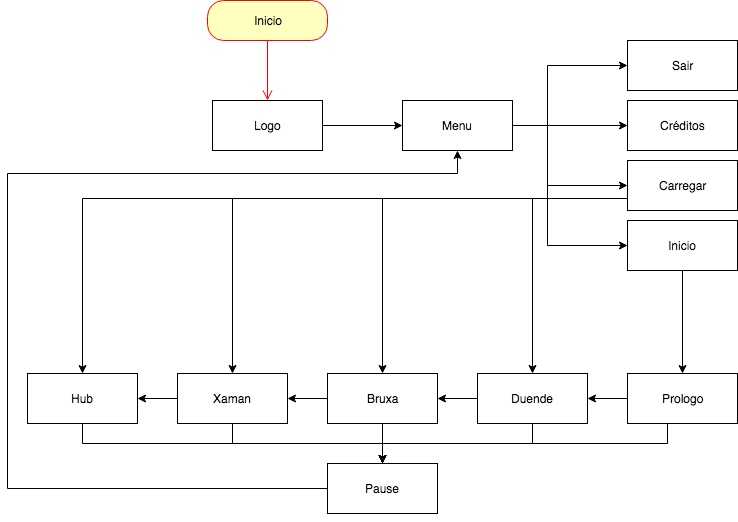
\includegraphics[width=\textwidth]{imagens/Flow.png} \end{center}
\legend{Fonte: Autoria Nossa} \end{figure}



\section{Estilo Estético}
O jogo será desenvolvido em 3D, utilizando-se a técnica conhecida como \textit{low poly}, que consiste em manter uma baixa contagem de polígonos na modelagem do jogo. Segundo \citeonline{GDCVault2:online} \footnote{Ethan Redd é Game Developer Independente, e palestrante da Game Developers Conference de 2017}, não existe uma delimitação forte demarcada para o que é considerado \textit{low poly}, mas ele define de forma não pragmática um modelo que tenha uma contagem menor que oito mil polígonos. Ainda afirma que existe uma série de vantagens em utilizar-se desse estilo estético, como maior produtividade e eficiência computacional, o que faz uma grande diferença quando se trabalha em times enxutos.

\begin{figure}[htb]
    \caption{\label{fig_lowpoly}Low Poly}
    \begin{center}
        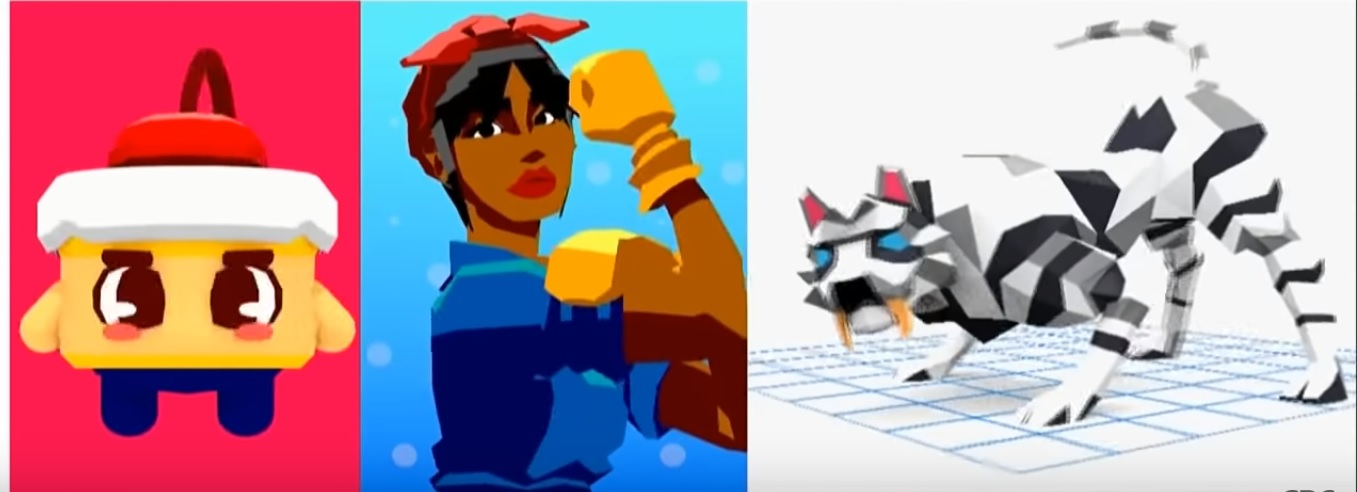
\includegraphics[width=\textwidth]{imagens/lowPoly.jpg}
    \end{center}
    \legend{Fonte: \citeauthoryear{GDCVault2:online}}
\end{figure}

Dito isso, cada uma das fases do jogo pretende retratar de forma aproximada os ambientes de origem dos personagens. Dessa forma, a paleta de cores e objetos encontrados em cada parte do jogo farão alusão a isso.

O mundo do Duende, ou \textit{Fulkominn}, palavra do islandês que significa ``perfeito'' \footnote{Segundo o site \citeonline{Icelandi31:online}}, foi baseada na vila de Geiranger da Noruega, que é uma pequena vila incrustada em um fiorde, com uma floresta a abraçando.


\begin{figure}[htb]
    \caption{\label{fig_mundoDuende}Geiranger - Noruega}
    \begin{center}
        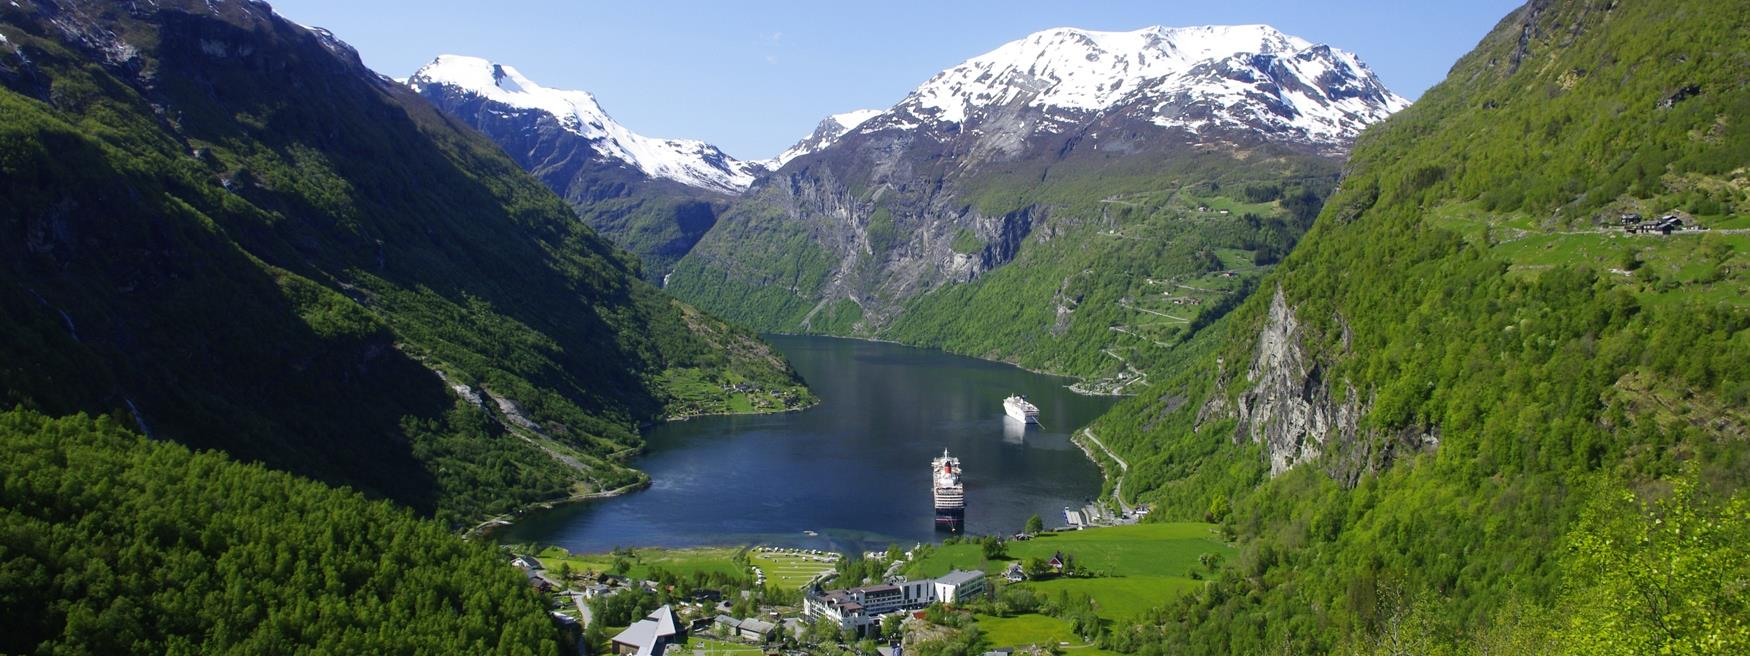
\includegraphics[width=\textwidth]{imagens/geiranger.jpeg}
    \end{center}
    \legend{Fonte: \citeauthoryear{Geirange16:online}}
\end{figure}

\clearpage

O mundo da Bruxa, foi baseado na cidade de Kilin no Reino Unido, um pequeno vilarejo que se ergue em uma planície escocesa e desemboca em um lago.



\begin{figure}[htb]
    \caption{\label{fig_mundoBruxa}Kilin - Reino Unido}
    \begin{center}
        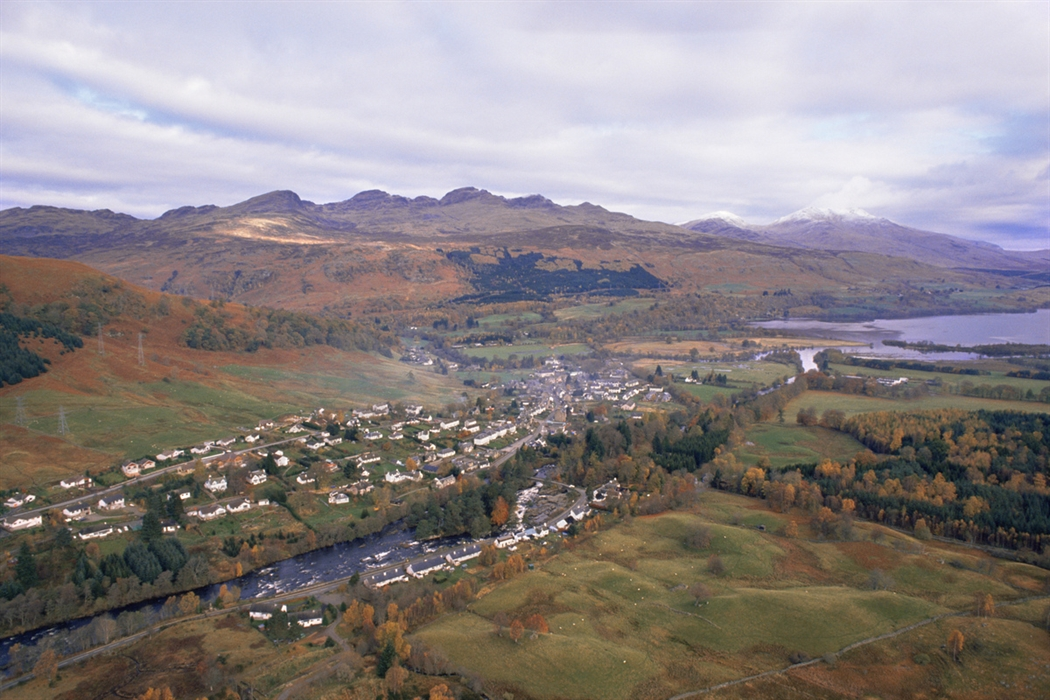
\includegraphics[width=0.9\textwidth]{imagens/kilin.jpg}
    \end{center}
    \legend{Fonte: \citeauthoryear{KillinVi68:online}}
\end{figure}

O mundo do Xamã foi inspirado pelos lugares em que os Pueblos ou Anasazi, viviam, tendo maior inspiração no Parque Nacional Mesa Verde, nos Estados Unidos.



\begin{figure}[htb]
    \caption{\label{fig_mundoXaman}Mesa Verde - Estados Unidos}
    \begin{center}
        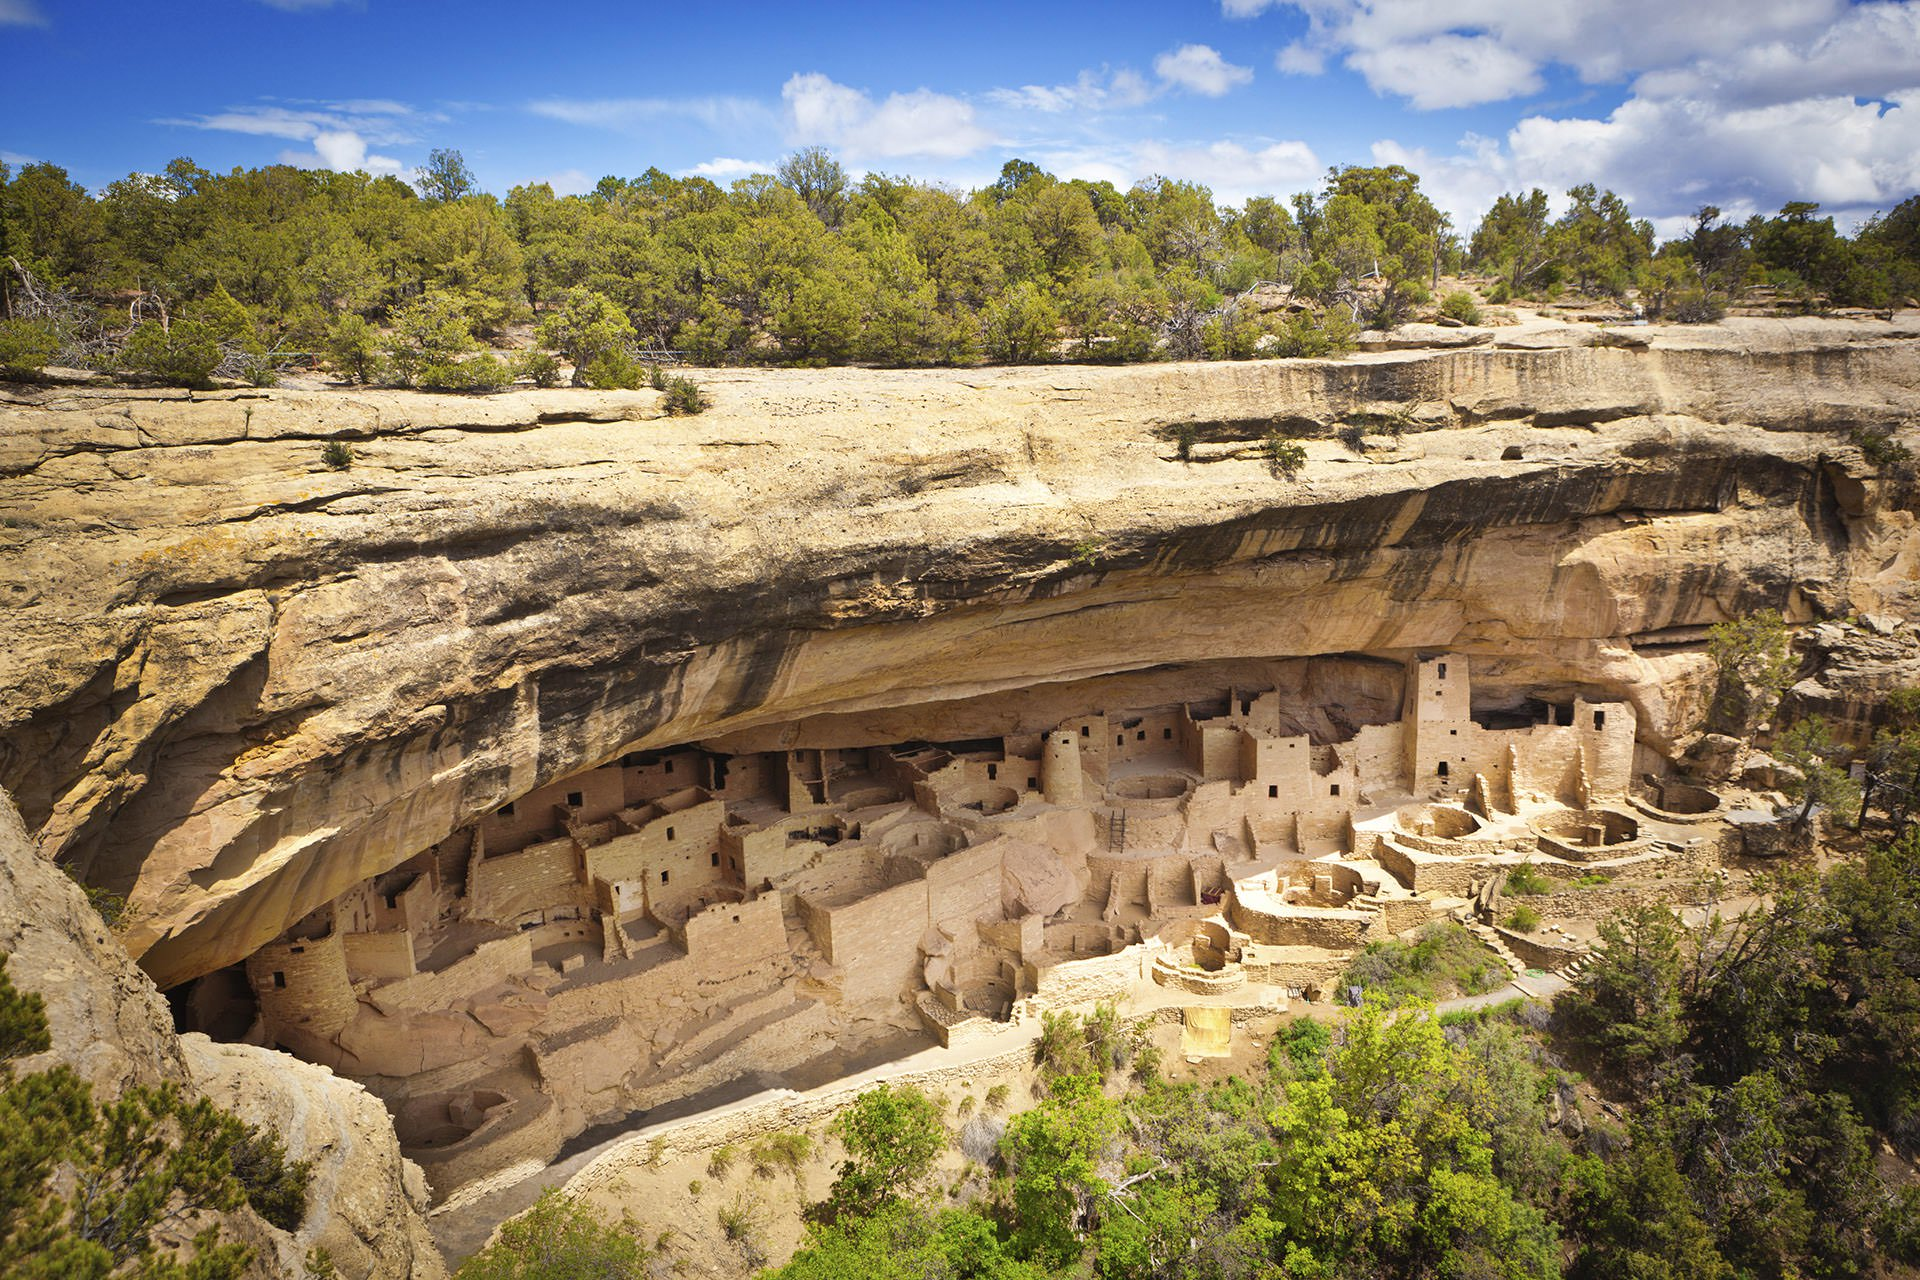
\includegraphics[width=\textwidth]{imagens/mesaverde.jpg}
    \end{center}
    \legend{Fonte: \citeauthoryear{MesaVerd44:online}}
\end{figure}



E por fim, a fase em que todos os elementos se unem, foi baseada no Parque Nacional de Tikal, na Guatemala, antiga formação de um templo Maia.


\begin{figure}[htb]
    \caption{\label{fig_mundoHub}Tikal - Guatemala}
    \begin{center}
        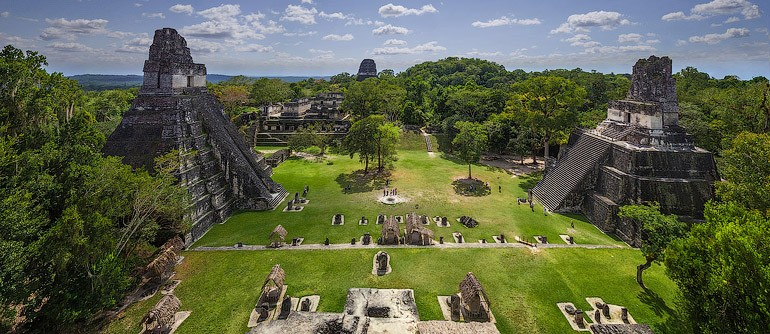
\includegraphics[width=\textwidth]{imagens/tikal.jpg}
    \end{center}
    \legend{Fonte: \citeauthoryear{MayaPyra92:online}}
\end{figure}

\clearpage

\section{Inspirações}


\subsection{Outlander}

Em 1945, em lua de mel na Escócia, a enfermeira em combate Claire Randall é misteriosamente transportada através do tempo para o ano de 1743.

Inspirou os cenários percorridos na fase da Bruxa, vestimentas dos personagens e a descrição psicológica da protagonista. Deu origem também a proposta de viagem no tempo utilizada pelo antagonista.

\begin{figure}[!htb] \caption{\label{Outlander}Outlander} \begin{center}
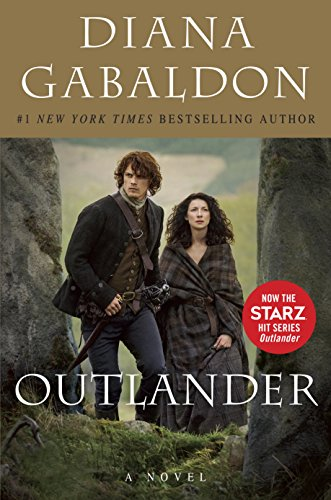
\includegraphics[width=0.6\textwidth]{imagens/outlander.jpg} \end{center}
\legend{Fonte: \citeauthoryear{gabaldon2004outlander}} \end{figure}

\clearpage

\subsection{Filha de Feiticeira}

Este romance de Celia Rees narra, em forma de diário, a história de Mary Nuttall, uma adolescente inglesa do século XVII que se vê obrigada a fugir para a América para não ter o mesmo destino de sua avó, condenada à forca sob acusação de feitiçaria.

A temática de caça às bruxas na Inglaterra inspirou o gameplay furtivo da bruxa, que não deve ser vista fazendo feitiços ou será condenada a forca.
A sequência desta história, Sangue de Feiticeira, conta a jornada de Mary já adulta casada com um nativo americano e vivendo dentro de sua cultura, o que inspirou também a construção do personagem Xamã.

\begin{figure}[!htb] \caption{\label{filha_feiticeira}Filha de Feiticeira}
    \begin{center}
    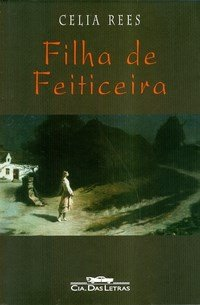
\includegraphics[width=0.6\textwidth]{imagens/feiticeira.jpeg} \end{center}
\legend{Fonte: \citeauthoryear{reesfilha}} \end{figure}

\clearpage

\subsection{Desencanto}

Bean é uma princesa que vive no reino mágico de Dreamland ao lado de Luci, seu demônio pessoal, e de Elfo, seu melhor amigo que a acompanham em sua jornada de alcoolismo, brigas de bar e descobertas inusitadas.

O desenho animado trouxe referências principalmente ao humor do jogo, facilitando uma linha de raciocínio a respeito de que tipo de piadas são bem aceitas pelo público. Trouxe também muitas referências à sobre a política e arquitetura da sociedade dos elfos que foram utilizadas na fase do duende.



\begin{figure}[!htb] \caption{\label{Desencanto}Desencanto} \begin{center}
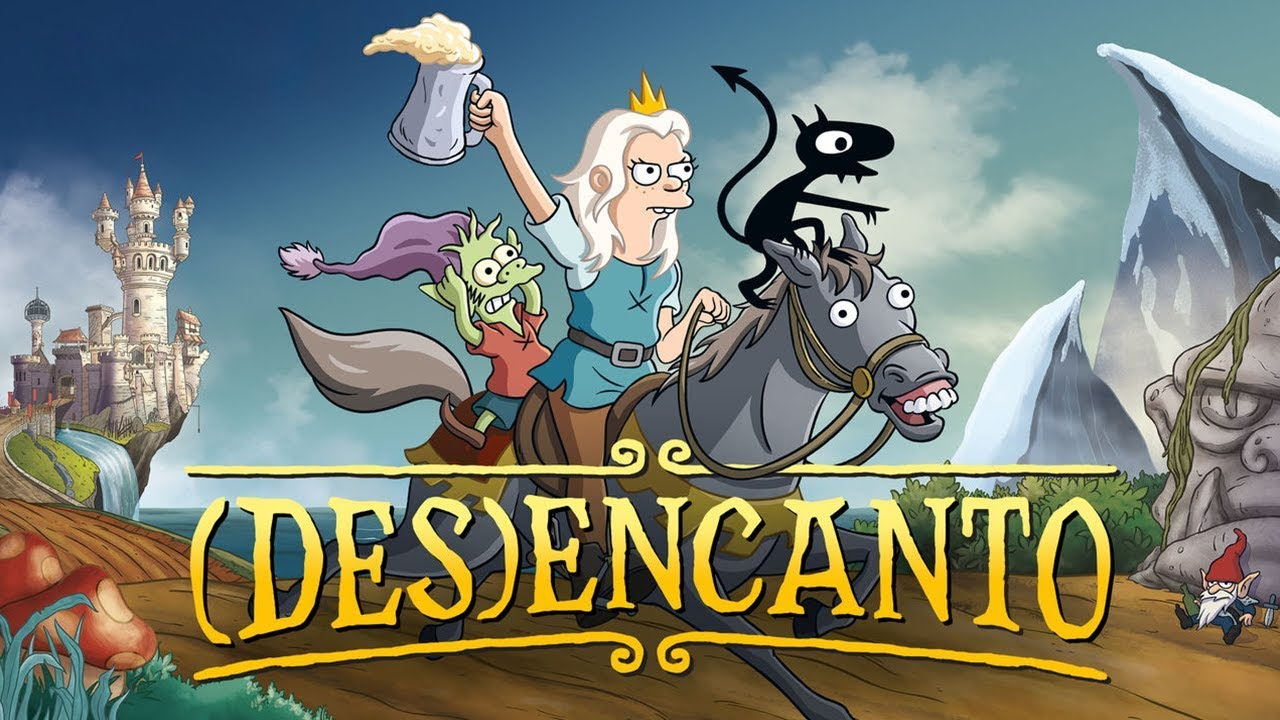
\includegraphics[width=\textwidth]{imagens/Desencanto.jpg} \end{center}
\legend{Fonte: \citeauthoryear{dessencanto}} \end{figure}

\clearpage

\subsection{Os Vingadores - Guerra infinita}

Neste filme da série Vingadores, os heróis enfrentam Thanos, que pretende juntar as joias do infinito para prosseguir com seu plano.

O filme deu origem a proposta do plano do antagonista: unir joias para potencializar sua magia. Assim como sua personalidade inflexível e sua presença imponente e temível.

\begin{figure}[!htb] \caption{\label{vingadores}Poster do Filme} \begin{center}

\includegraphics[width=0.6\textwidth]{imagens/vingadores.jpeg} \end{center}
\legend{Fonte: \citeauthoryear{avengers}} \end{figure}

\clearpage

\subsection{Franquia God of War}
A franquia conta a história de Kratos, um personagem que foi enganado pelos deuses do Olimpo, e está em busca de sua vingança.

A franquia inspirou todo o gameplay assim como a movimentação de câmera. O level design segue uma maneira completamente linear e a câmera acompanha o personagem sem que possa ser movimentada pelo jogador.

\begin{figure}[!htb] \caption{\label{god_of_war}God of War} \begin{center}
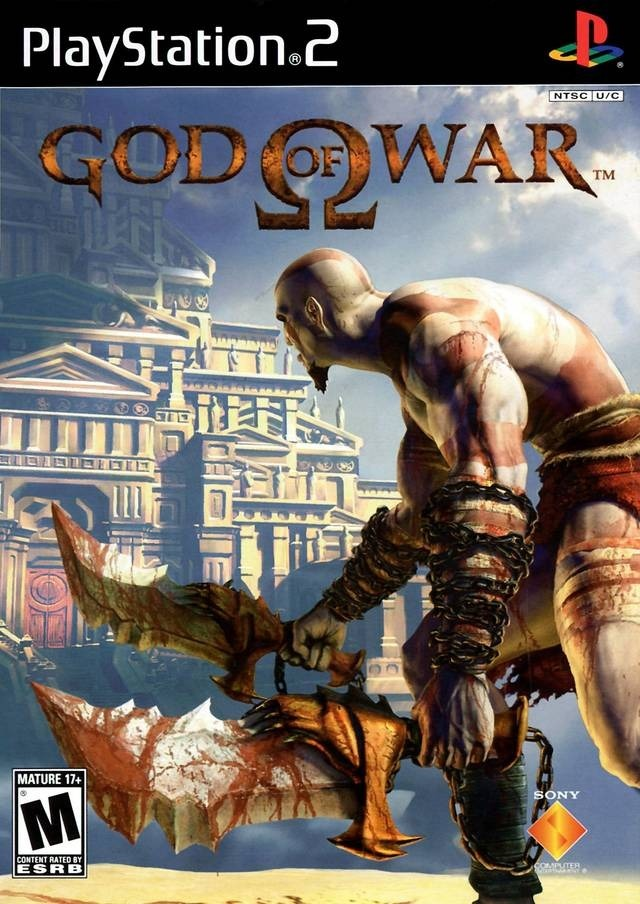
\includegraphics[width=0.6\textwidth]{imagens/GodofWar.jpg} \end{center}
\legend{Fonte: \citeauthoryear{godofwar}} \end{figure}

\clearpage

\subsection{Brownies}

São pequenos seres noturnos do folclore britânico, que cuidam dos afazeres da casa, se ofendem facilmente e evitam serem vistos pelos humanos \cite{britannica_2011, carolyn_2016}.

A lenda inspirou o gameplay furtivo da fase do duende, que não deve ser visto por humanos assim como a personalidade explosiva do protagonista.

\begin{figure}[!htb]
    \caption{\label{fig_brownie}\textbf{Brownie} por Arthur Rackham }
    \begin{center} 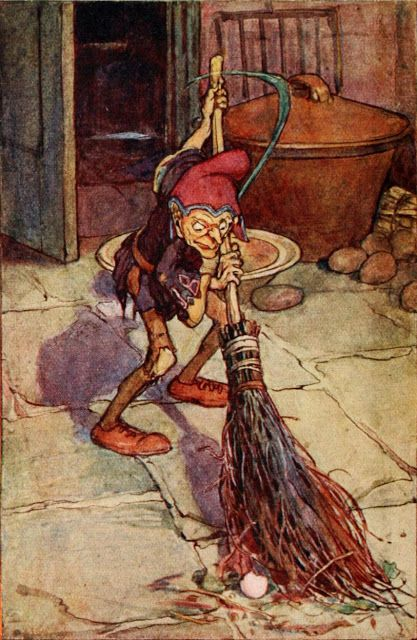
\includegraphics[width=0.6\textwidth]{imagens/brownie.jpg}
    \end{center} \legend{Fonte: \citeauthoryear{carolyn_2016}} \end{figure}

\clearpage


\subsection{Alux}

Alux são pequenas criaturas da mitologia de alguns povos Maias, costumeiramente
são invisíveis, mas podem se tornar visíveis para se comunicar e assustar
humanos. 

\begin{citacao}
``When given food, drink, and ritual homage, the aluxo'b protect the farmer’s crops from hungry animals. [\ldots] The aluxo'b summon strong winds, emit piercing whistling sounds, and propel stones at intruders.'' 
\cite{storniolo2009out} \footnote{Quando recebem comida, bebida e
um ritual de homenagem, o alux protegerá a plantação do fazendeiro de
animais famintos. [\ldots] O alux invoca fortes ventos, emite agudos sons
sibilantes, e lança pedras em intrusos: Tradução nossa}
\end{citacao}


\begin{figure}[!htb] \caption{\label{fig_alux}Alux} \begin{center}
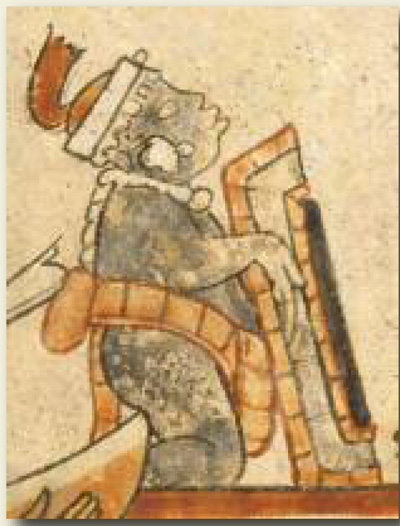
\includegraphics[width=0.6\textwidth]{imagens/alux.jpg} \end{center}
\legend{Fonte:~\citeauthoryear{storniolo2009out}} \end{figure}

\clearpage

\subsection{Pueblos}

Pueblos foi  um povo que habitou o que hoje é o sudoeste dos Estados Unidos, mais especificamente a região de Colorado, Utah, Novo México, e Arizona.\cite{civPerdidas2017,lyneis1995virgin} Acredita-se que são antepassados de diversas tribos norte americanas como Ute, Zuni, Navajo e Hopi, e que essas tribos ainda pratiquem seus rituais. Pela região que habitam, grande parte de seus ritos ocorriam para os deuses da chuva\cite{abreu94}.

Os rastros desse povo inspiraram a arquitetura da fase do Xamã, bem como sua personalidade, vestimentas e ações.

\begin{figure}[!htb] \caption{\label{fig_puebloan}Construção Pueblo} \begin{center}
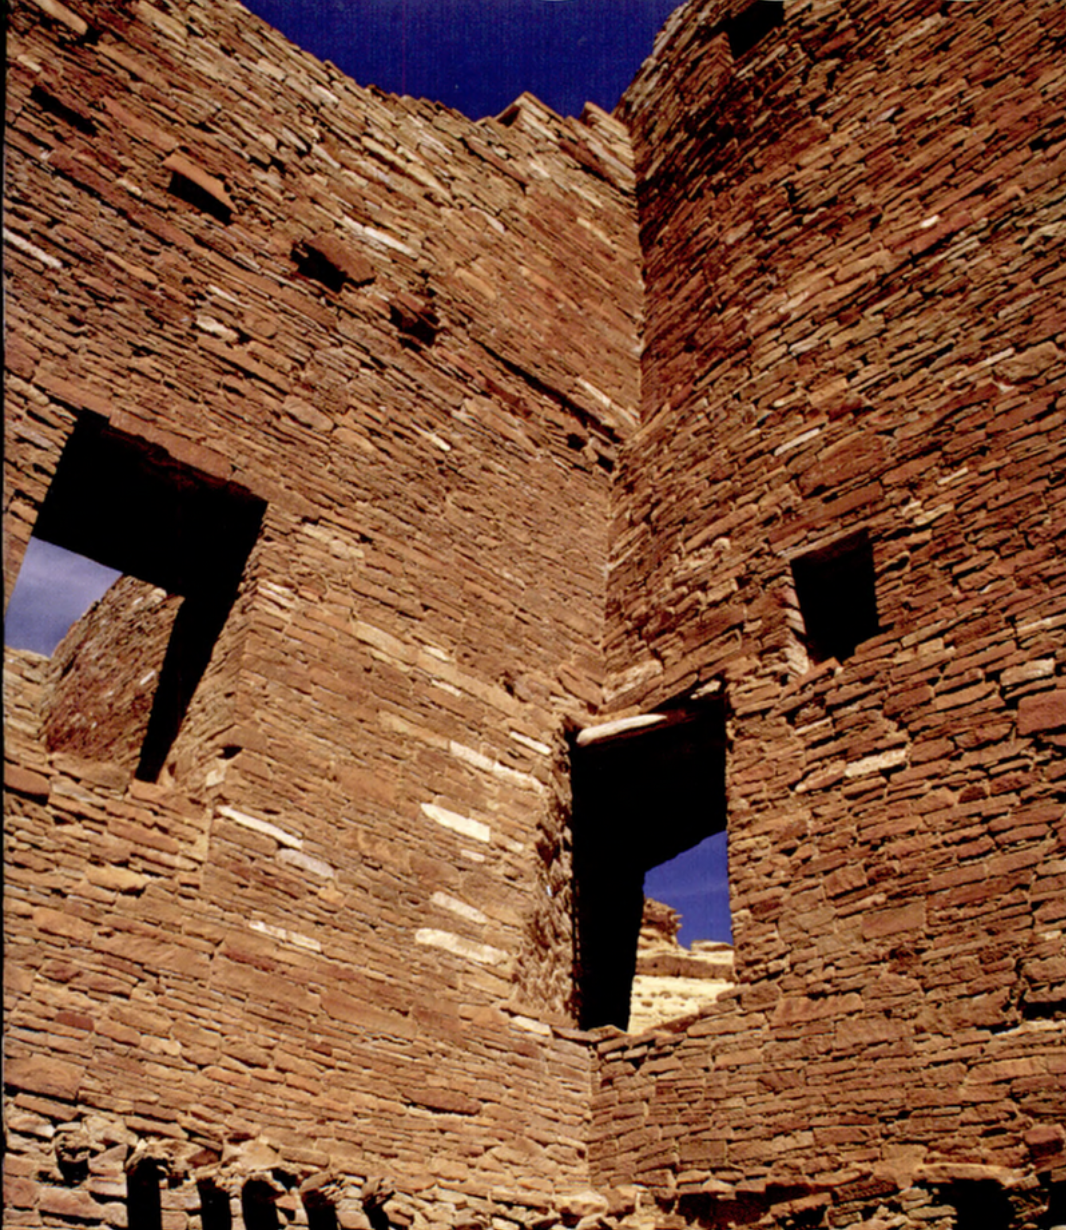
\includegraphics[width=\textwidth]{imagens/puebloans.png} \end{center}
\legend{Fonte:~\citeauthoryear{heyder1997anasazi}} \end{figure}

\clearpage

\subsection{Siempre Bruja}

A série que conta a história de uma bruxa negra e escrava que é transportada pelo tempo para enfrentar um grande bruxo.

A série inspirou uma visão menos explorada das bruxas, isto é, sem chapeis pontudos ou rostos desproporcionais. Carmen, a protagonista, trouxe uma perspectiva mais próxima da nossa realidade uma vez que é uma bruxa latina, inspirando itens, poderes e trazendo novas ideias para a proposta de viagem no tempo que compõe grande parte do enredo deste jogo.

\begin{figure}[!htb] \caption{\label{siempre}Siempre Bruja} \begin{center}
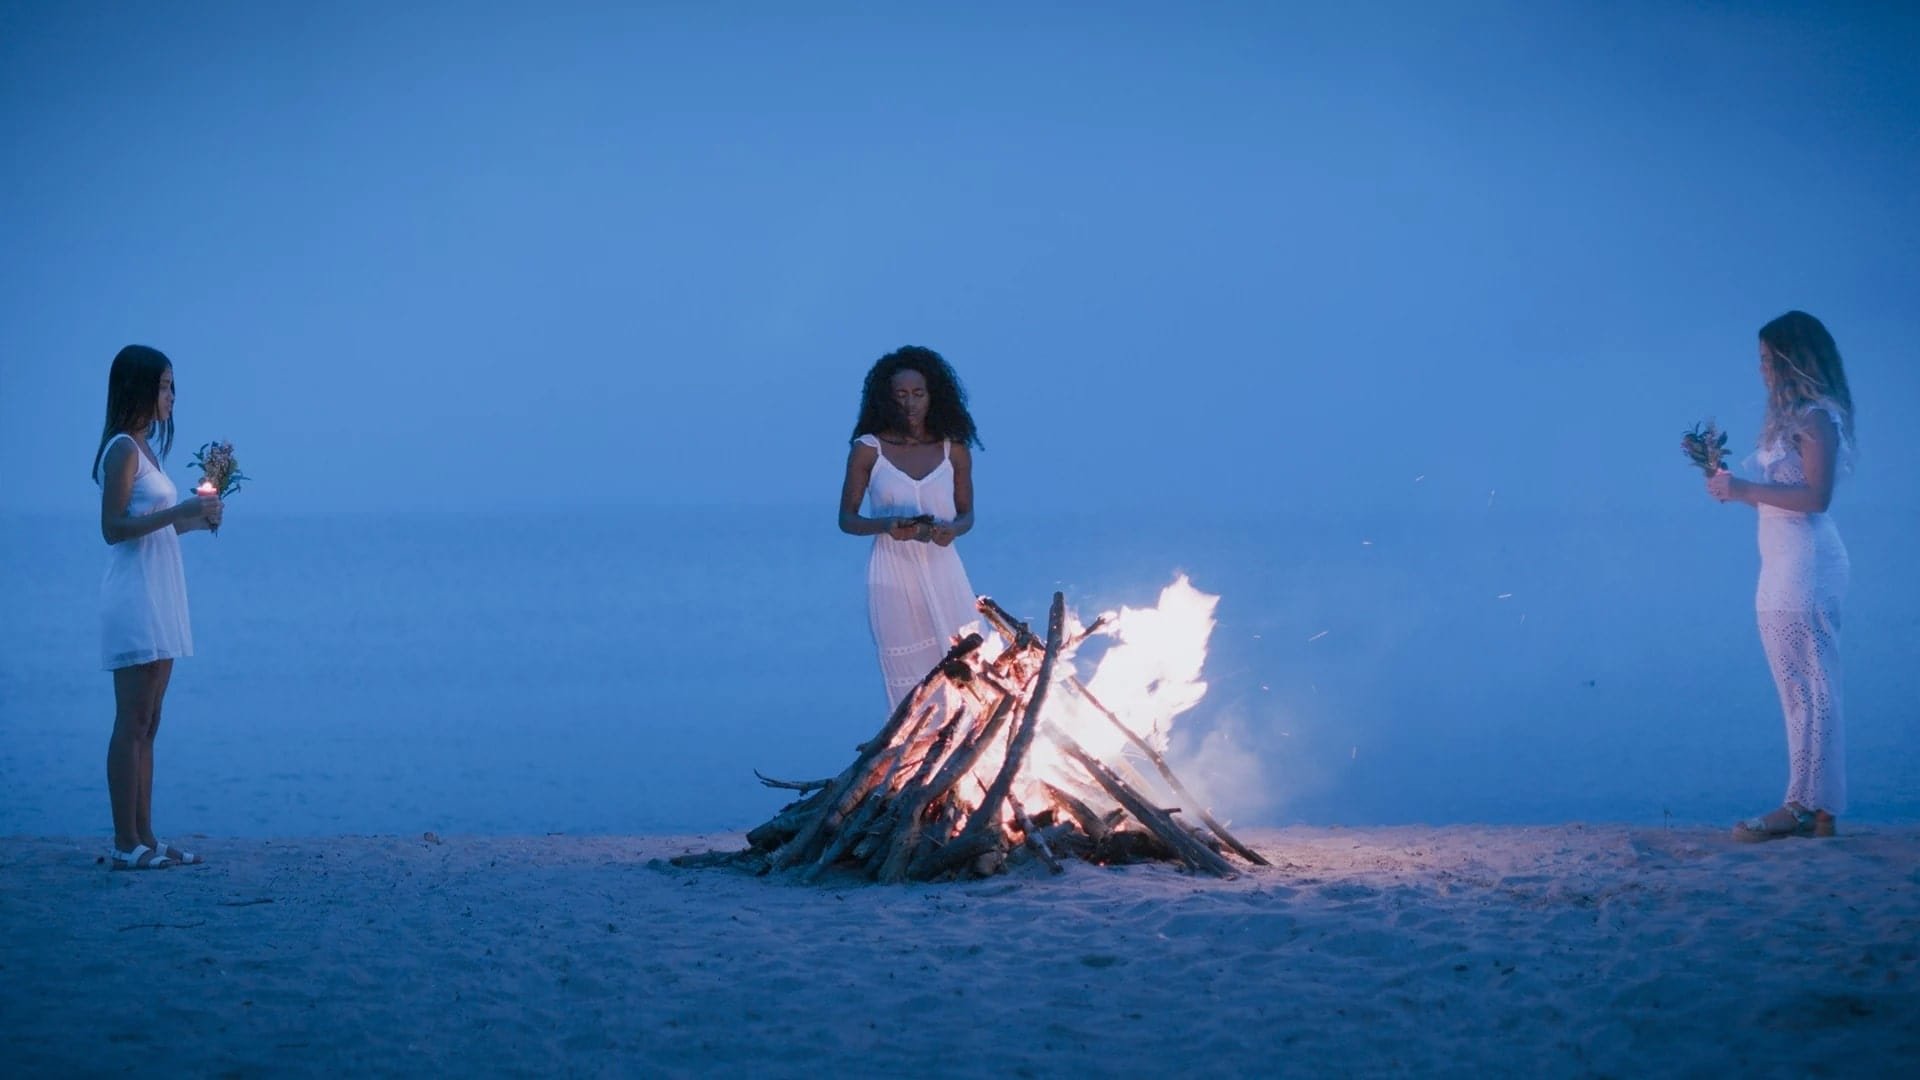
\includegraphics[width=\textwidth]{imagens/SiempreBruja.jpg} \end{center}
\legend{Fonte: \citeauthoryear{siempre}} \end{figure}

\clearpage

\subsection{\textit{The Ghost of a Tale}} Segundo o site do jogo (\citeyear{Ghostofa36:online})  ``Você é Tilo,
um corajoso rato menestrel em uma arriscada missão para achar seu verdadeiro
amor. Use sua furtividade e destreza para explorar o Forte \textit{Dwindling
Heights}''

Trouxe muitas dicas sobre furtividade e exploração para o gameplay deste jogo, além de uma animação cativante que procuramos imitar.

\begin{figure}[!htb] \caption{\label{tale}The Ghost of a Tale} \begin{center}
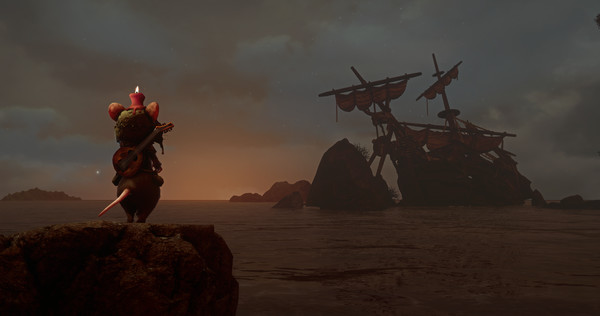
\includegraphics[width=\textwidth]{imagens/tale.jpg} \end{center}
\legend{Fonte: \citeauthoryear{Ghostofa36:online}} \end{figure}

\clearpage

\subsection{\textit{Moss}}
Em Moss, você ajuda o pequeno roedor Quill, a passar por muitos desafios para salvar seu tio. \cite{Moss18}

Inspirou os cenários de várias fases deste jogo. O uso de uma palheta de cores rica em tons de verde e azul é muito agradável e transmite muito bem o clima de magia e natureza que queremos transmitir. 

\begin{figure}[!htb] \caption{\label{fig_moss}Moss} \begin{center}
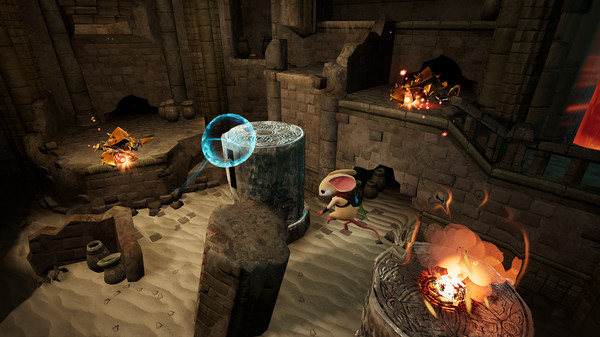
\includegraphics[width=\textwidth]{imagens/moss.jpg} \end{center}
\legend{Fonte: \citeauthoryear{Moss18}} \end{figure}

\clearpage

\subsection{\textit{Zelda: Windwaker}}
\textit{The Legend of Zelda: The Wind Waker} é um jogo de ação-aventura, desenvolvido pela \textit{Nintendo Entertainment Analysis \& Development} e publicado pela Nintendo para o Nintendo \textit{GameCube}.

O jogo trás como inspiração seu visual cartunesco e \textit{low poly}, com uma seleção de cores e ambientes agradável.

\begin{figure}[!htb] \caption{\label{fig_zelda}Legend of Zelda: Wind Waker} \begin{center}
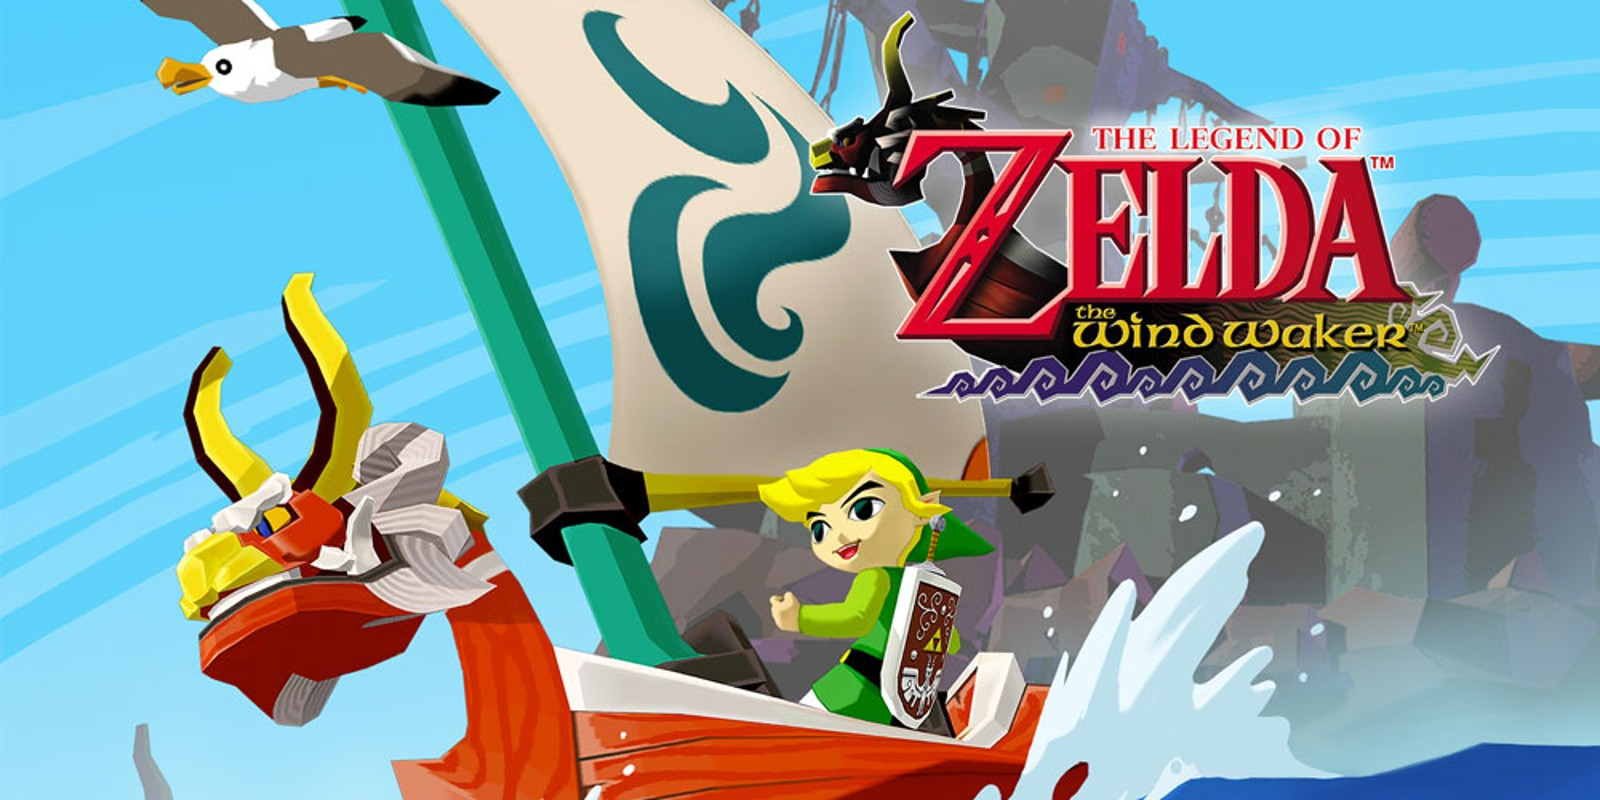
\includegraphics[width=\textwidth]{imagens/windwaker.jpeg} \end{center}
\legend{Fonte: \citeauthoryear{zeldaWind}} \end{figure}

\clearpage

\section{Equipe de Desenvolvimento}

\subsection{Logo}

~

\begin{figure}[!htb] \caption{\label{fig_logo}Logo Cygnus Studio} \begin{center}
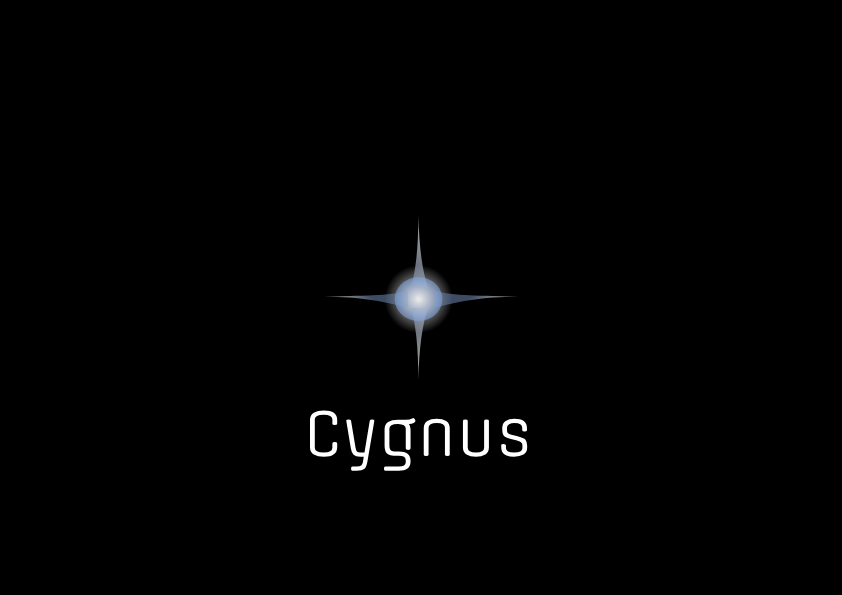
\includegraphics[width=0.5\textwidth]{imagens/logo.png}\end{center}
\legend{Fonte: Autoria Nossa} \end{figure}

\subsection{Slogan}

Mirando as estrelas

\subsection{Divisão de tarefas}

A equipe dividiu-se de forma a
otimizar as forças de cada um dos integrantes, desta forma ficamos com a
seguinte divisão de tarefas não rígidas:

\begin{quadro}[htb] \caption{\label{quadro_atuacao}Atuação da equipe}
    \begin{tabularx}{\textwidth}{|c|X|} \hline \textbf{Nome} &
        \textbf{Atuação}\\ \hline Marina & Game Design Construção de
        Personagens, Construção de mundo, Design de personagens, Arte Conceitual
        \\ \hline Eric   & Construção de Personagens, Construção de mundo, Arte
        Técnica, Programação                                        \\ \hline
        Pedro  & Construção de Personagens, Construção de mundo, Arte Técnica,
        Programação \\ \hline \end{tabularx} \fonte{Autoria Nossa}
\end{quadro}
